% 3,5,6,7,8

%\pagebreak

\aufgabe{Attempt any 10 questions}{20}

According to the NASA Managers, the Space shuttle Challenger had a failure rate of 1 in 100000. However Richard Feynman who was investigating the bursting of the space shuttle that led to the killing of all crew members, reported a failure rate of 1 in 200. 
What is the MTTF in both the cases?


Calculate 

You are asked to design a real time distributed network with 3 nodes. All the nodes are equipped with a low speed CAN controller ( TJA1054T ) and a host CPU as shown in the figure. Pin Number 16 and Pin number 17 are the Can Rx and Can Tx pins on the host CPU respectively.
%\begin{figure}[ht]
%\begin{center}
$\begin{array}{cc}
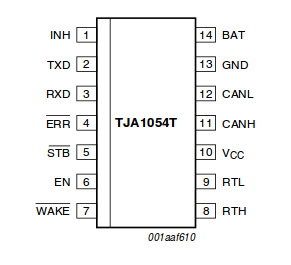
\includegraphics[width=6cm]{master-exam-2016/tja1054t} &
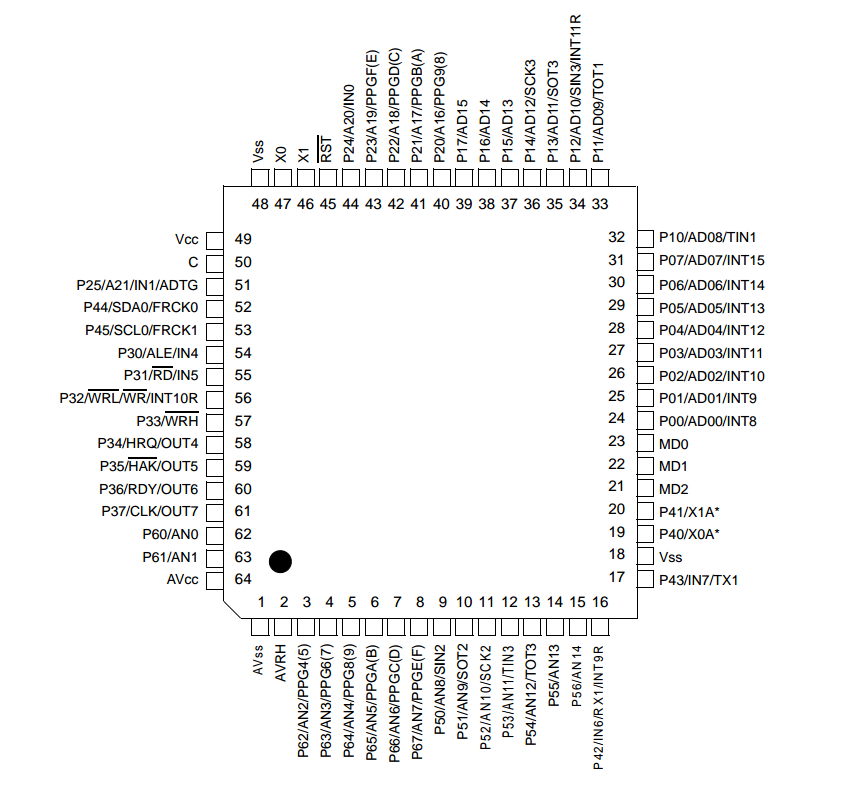
\includegraphics[width=8cm]{master-exam-2016/fujitsu}
\end{array}$
%\end{center}
%\end{figure}

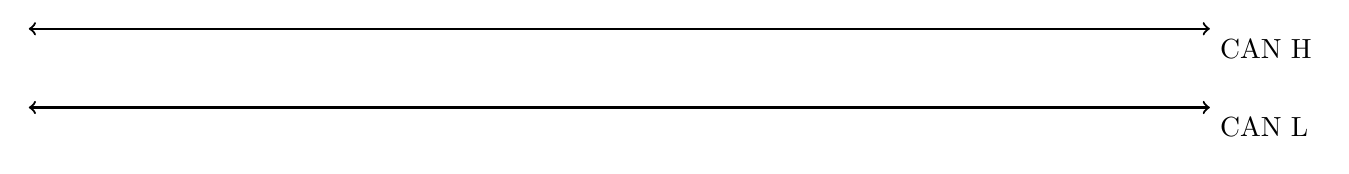
\begin{tikzpicture}
\draw[thick,<->] (0,10) -- (15,10) node[anchor=north west] {CAN L};
\draw[thick,<->] (0,11) -- (15,11) node[anchor=north west] {CAN H};;
\end{tikzpicture}

\begin{enumerate}
    \item Draw how a real time node looks like and list the main components in such a node.
    \item In the fig above, connect the CAN receive and transmit pins on the host CPU with those on the communication controller.
    \item In the fig above, connect the communication bus with the appropriate pins on the communication controller.
    \item Now, in the page below, make a new distributed network diagram with 3 nodes by connecting all of them with each other via the communication bus.
    \item Assign a CAN ID to each node and discuss how the nodes access the bus in case of collisions?
\end{enumerate}

\pagebreak

\headheight = 78pt

\begin{tikzpicture}
\node (rect) at (0,0) [draw, text width=16.6 cm, minimum height=24cm]{};
\node[below right, text width=16.6 cm] at (rect.north west) {
    \lsg{
\begin{tikzpicture}[squarednode/.style={rectangle, draw=red!60, fill=red!5, very thick, minimum size=5mm}]
%Nodes
\node[squarednode]      (hostcpu)                              {2};
\node[squarednode]      (coummunication)                              {4};
%\node[roundnode]        (uppercircle)       [above=of maintopic] {1};
%Lines
\draw[->] (coummunication.south) -- (hostcpu.north);
%\draw[->] (maintopic.east) -- (rightsquare.west);
%\draw[->] (rightsquare.south) .. controls +(down:7mm) and +(right:7mm) .. (lowercircle.east);
\end{tikzpicture}
    }
   };
\end{tikzpicture}


Each node is connected in parallel to a 12V DC battery with a capacity of 5400 mAh. Each node has an energy consumption of 100 mAh in operational mode and 1 mAh in standby mode.

\begin{enumerate}
    \addtocounter{enumi}{5}
%    \setcounter{enumii}{4}
    \item Extend your block diagram above by connecting the battery unit to the nodes.
    \item Assuming that the car has no charger unit, how much energy does the battery still have after 20 hours, if the car is in the operational mode for 15 hours and in standby mode for 5 hours ?
\end{enumerate}

\begin{tikzpicture}
\node (rect) at (0,0) [draw, text width=16.6 cm, minimum height=5cm]{};
\node[below right, text width=16.6 cm] at (rect.north west) {
    \lsg{
    Please sketch a model here
    }
   };
\end{tikzpicture}


Assuming Node 3, starts sending Error Frames on the bus. 
\begin{enumerate}
    \addtocounter{enumi}{7}
    \item How does the CAN driver know about the error frames on the bus and what measures would you take to make sure that all the nodes can still communicate with each other? Hint > Please see the chip diagram.
    \item Discuss why a terminating resistance is important in a multi-node communication network system.
\end{enumerate}

\begin{tikzpicture}
\node (rect) at (0,0) [draw, text width=16.6 cm, minimum height=6cm]{};
\node[below right, text width=16.6 cm] at (rect.north west) {
    \lsg{
    Please sketch a model here
    }
   };
\end{tikzpicture}
 

The two farthest nodes are 5 m away from each other. The low speed CAN transciever can transmit and receive messages with a bandwidth of 125 KBit / second. The speed of the transmission of the bits is 2/3 of the speed of the light and the message length is 100 bits.

\begin{enumerate}
    \addtocounter{enumi}{9}
    \item What is the bit length of the two farthest nodes? 
    \item Calculate the best channel utilization in percentage.
\end{enumerate}

\begin{tikzpicture}
\node (rect) at (0,0) [draw, text width=16.6 cm, minimum height=6cm]{};
\node[below right, text width=16.6 cm] at (rect.north west) {
    \lsg{
    Please sketch a model here
    }
   };
\end{tikzpicture}


TDMA is Time Division Multiple Access and CSMA/CA is Carrier Sense Multiple Access / Collision Avoidance. 

\begin{enumerate}
    \addtocounter{enumi}{11}
    \item Name 5 important parameters which you would need to know, before choosing the right protocol such as the one above
\end{enumerate}

\begin{tikzpicture}
\node (rect) at (0,0) [draw, text width=16.6 cm, minimum height=6cm]{};
\node[below right, text width=16.6 cm] at (rect.north west) {
    \lsg{
    Please sketch a model here
    }
   };
\end{tikzpicture}

\pagebreak

\aufgabe{}{10}


You are given a quartz which oscillates at the rate of 32768 ticks per second. 

Your job is to make 3 local clocks each with a macro-granularity of 512 ticks. Each clock drifts differently at a drift rate $\rho$ $10^{-9}$ s/s, $2*10^{-9}$ s/s, $3*10^{-9}$ s/s respectively.

\begin{enumerate}
    \addtocounter{enumi}{0}
\item What is the granularity of the reference clock?
\item What is the granularity of the local clock?
\item What is the minimum time and the maximum time that can be measured in one of the local clock with a 32 bit variable?
\item What is the precision of the clock ensemble over an interval of interest of 1 second?
\end{enumerate}

\begin{tikzpicture}
\node (rect) at (0,0) [draw, text width=16.6 cm, minimum height=13cm]{};
\node[below right, text width=16.6 cm] at (rect.north west) {
    \lsg{
    Please sketch a model here
    }
   };
\end{tikzpicture}

The clocks are synchronized to the reference clock via a communication bus. The latency jitter between the the reference clock and the local clock is $10^{-12}$ s.
The formula for drift offset is $\Gamma =  2 * \rho * R_{int}$

\begin{enumerate}
    \addtocounter{enumi}{4}
\item Calculate the synchronization interval according the central master algorithm of one of the local clock of your choice.

\end{enumerate}

\begin{tikzpicture}
\node (rect) at (0,0) [draw, text width=16.6 cm, minimum height=6 cm]{};
\node[below right, text width=16.6 cm] at (rect.north west) {
    \lsg{
    Please sketch a model here
    }
   };
\end{tikzpicture}

\aufgabe{}{10}

Consider a combustion engine with an injection valve. The start point of fuel injection must be precise within $2\degree$ of the measured angular crankshaft position.
\begin{enumerate}
\item Calculate the temporal accuracy of the system, if the crankshaft revolves with 6000 rpm.
\end{enumerate}

\begin{tikzpicture}
\node (rect) at (0,0) [draw, text width=16.6 cm, minimum height=7cm]{};
\node[below right, text width=16.6 cm] at (rect.north west) {
    \lsg{
    Please sketch a model here
    }
   };
\end{tikzpicture}

Considering an update rate $d_{update}$ of 10 $\mu$s, WCET of the sender as 500 ns and the WCET of the receiver as 1500 ns and the worst case latency of the communication bus as 18 $\mu$s, discuss the type of the image derived ( phase sensitive or phase insensitive ).

\begin{enumerate}
\addtocounter{enumi}{1}
\item Discuss the type of the image if the high level PAR protocol of the RT transaction between the sender and the receiver allows a maximum of 2 retry.
\item How can you solve the problem of phase insensitive images?
\end{enumerate}


\begin{tikzpicture}
\node (rect) at (0,0) [draw, text width=16.6 cm, minimum height=15cm]{};
\node[below right, text width=16.6 cm] at (rect.north west) {
    \lsg{
    Please sketch a model here
    }
   };
\end{tikzpicture}

\pagebreak

\aufgabe{}{20}

Consider a task set T composed of the following three periodic tasks:
\begin{itemize}
\item T1(0, 1, 6) (release time, computation time, deadline)
\item T2(0, 2, 10)
\item T3(0, 5, 15)
\end{itemize}

\begin{enumerate}
\item Compute the major cycle of the task set. 
\item Verify the schedulability under the EDF algorithm. 
\item Build the schedule.
\end{enumerate}

Consider the following aperiodic tasks:
\begin{itemize}
    \item T4(1, 2, 29) (release time, computation time, deadline)
    \item T5(13, 2, 10)
    \item T6(21, 4, 9)
\end{itemize}

\begin{enumerate}
\addtocounter{enumi}{3}
\item \textbf{\underline{All}} aperiodic tasks are scheduled in the background together with the main tasks. Compute the response times of tasks T4, T5, and T6. 
\item Do you think that any of the aperiodic task would not be able to meet the deadline?
\end{enumerate}
